\documentclass[]{usiinfbachelorproject}
\usepackage{subfigure}
\usepackage{float}

\captionsetup{labelfont={bf}}

\author{Marco Bedulli}

\title{CSI:Cube8}
\subtitle{Augmenting Software System Representation with Corollary Information}
\versiondate{\today}

\begin{committee}
%With more than 1 advisor an error is raised...: only 1 advisor is allowed!
\advisor[Universit\`a della Svizzera Italiana, Switzerland]{Prof.}{Michele}{Lanza}
%You can comment out  these lines if you don't have any assistant
\assistant[Universit\`a della Svizzera Italiana, Switzerland]{Phd.}{Luca}{Ponzanelli}
%\assistant[Universit\`a della Svizzera Italiana, Switzerland]{Dot.}{Andrea}{Mocci}

\end{committee}

\abstract {
The information not strictly related to a software system, likes forum discussions and code documentation, can be useful to understand how much knowledge is available about the source code. Using an augmented city metaphor as visualization method we allow the developer to evaluate the information coverage. A developer is thus able to visualize which part needs more documentation and also directly access the online information related to it.


}


\begin{document}
\maketitle
\tableofcontents

\pagebreak
\listoffigures

\pagebreak

%%%%%%%%%%%%%%%%%%%%%%%%%
\section{Introduction} \label{introduction}

The main purpose of this paper is offering to anyone a way to get an impression at first glance about the information coverage of a software in an immediate and intuitively way. It can be seen as the combination of the needs to get a better understanding of the backbones in a project and the needs to find all the available information related to it rendered in a easy and fast system.

Since the web community has plenty of features questions and answers on a wide range of topics in computer programming, having a pre-built application able to show the most popular discussion tightly focused on a specific problem could undoubtedly reduce the amount of time spent on learning all the functionality of the project.



\subsection{City metaphor as visualization method } 


The city is create using a mix of information related and not to the code that are mapped to construct the building of the city.
The use of a metaphor from the physical world is the key point that makes this system particularly intuitive and effective. In fact, it allows the viewer to transfer existing perceptual abilities to the comprehension of the visualization.\\
R. P. Gabriel \cite{gabry} said that "Habitability is the characteristic of source code that enables programmer, code ,bag-fixer, and people coming to the code later in life to understand his construction and his intentions[..]". 
\begin{figure}[h]
	\centering
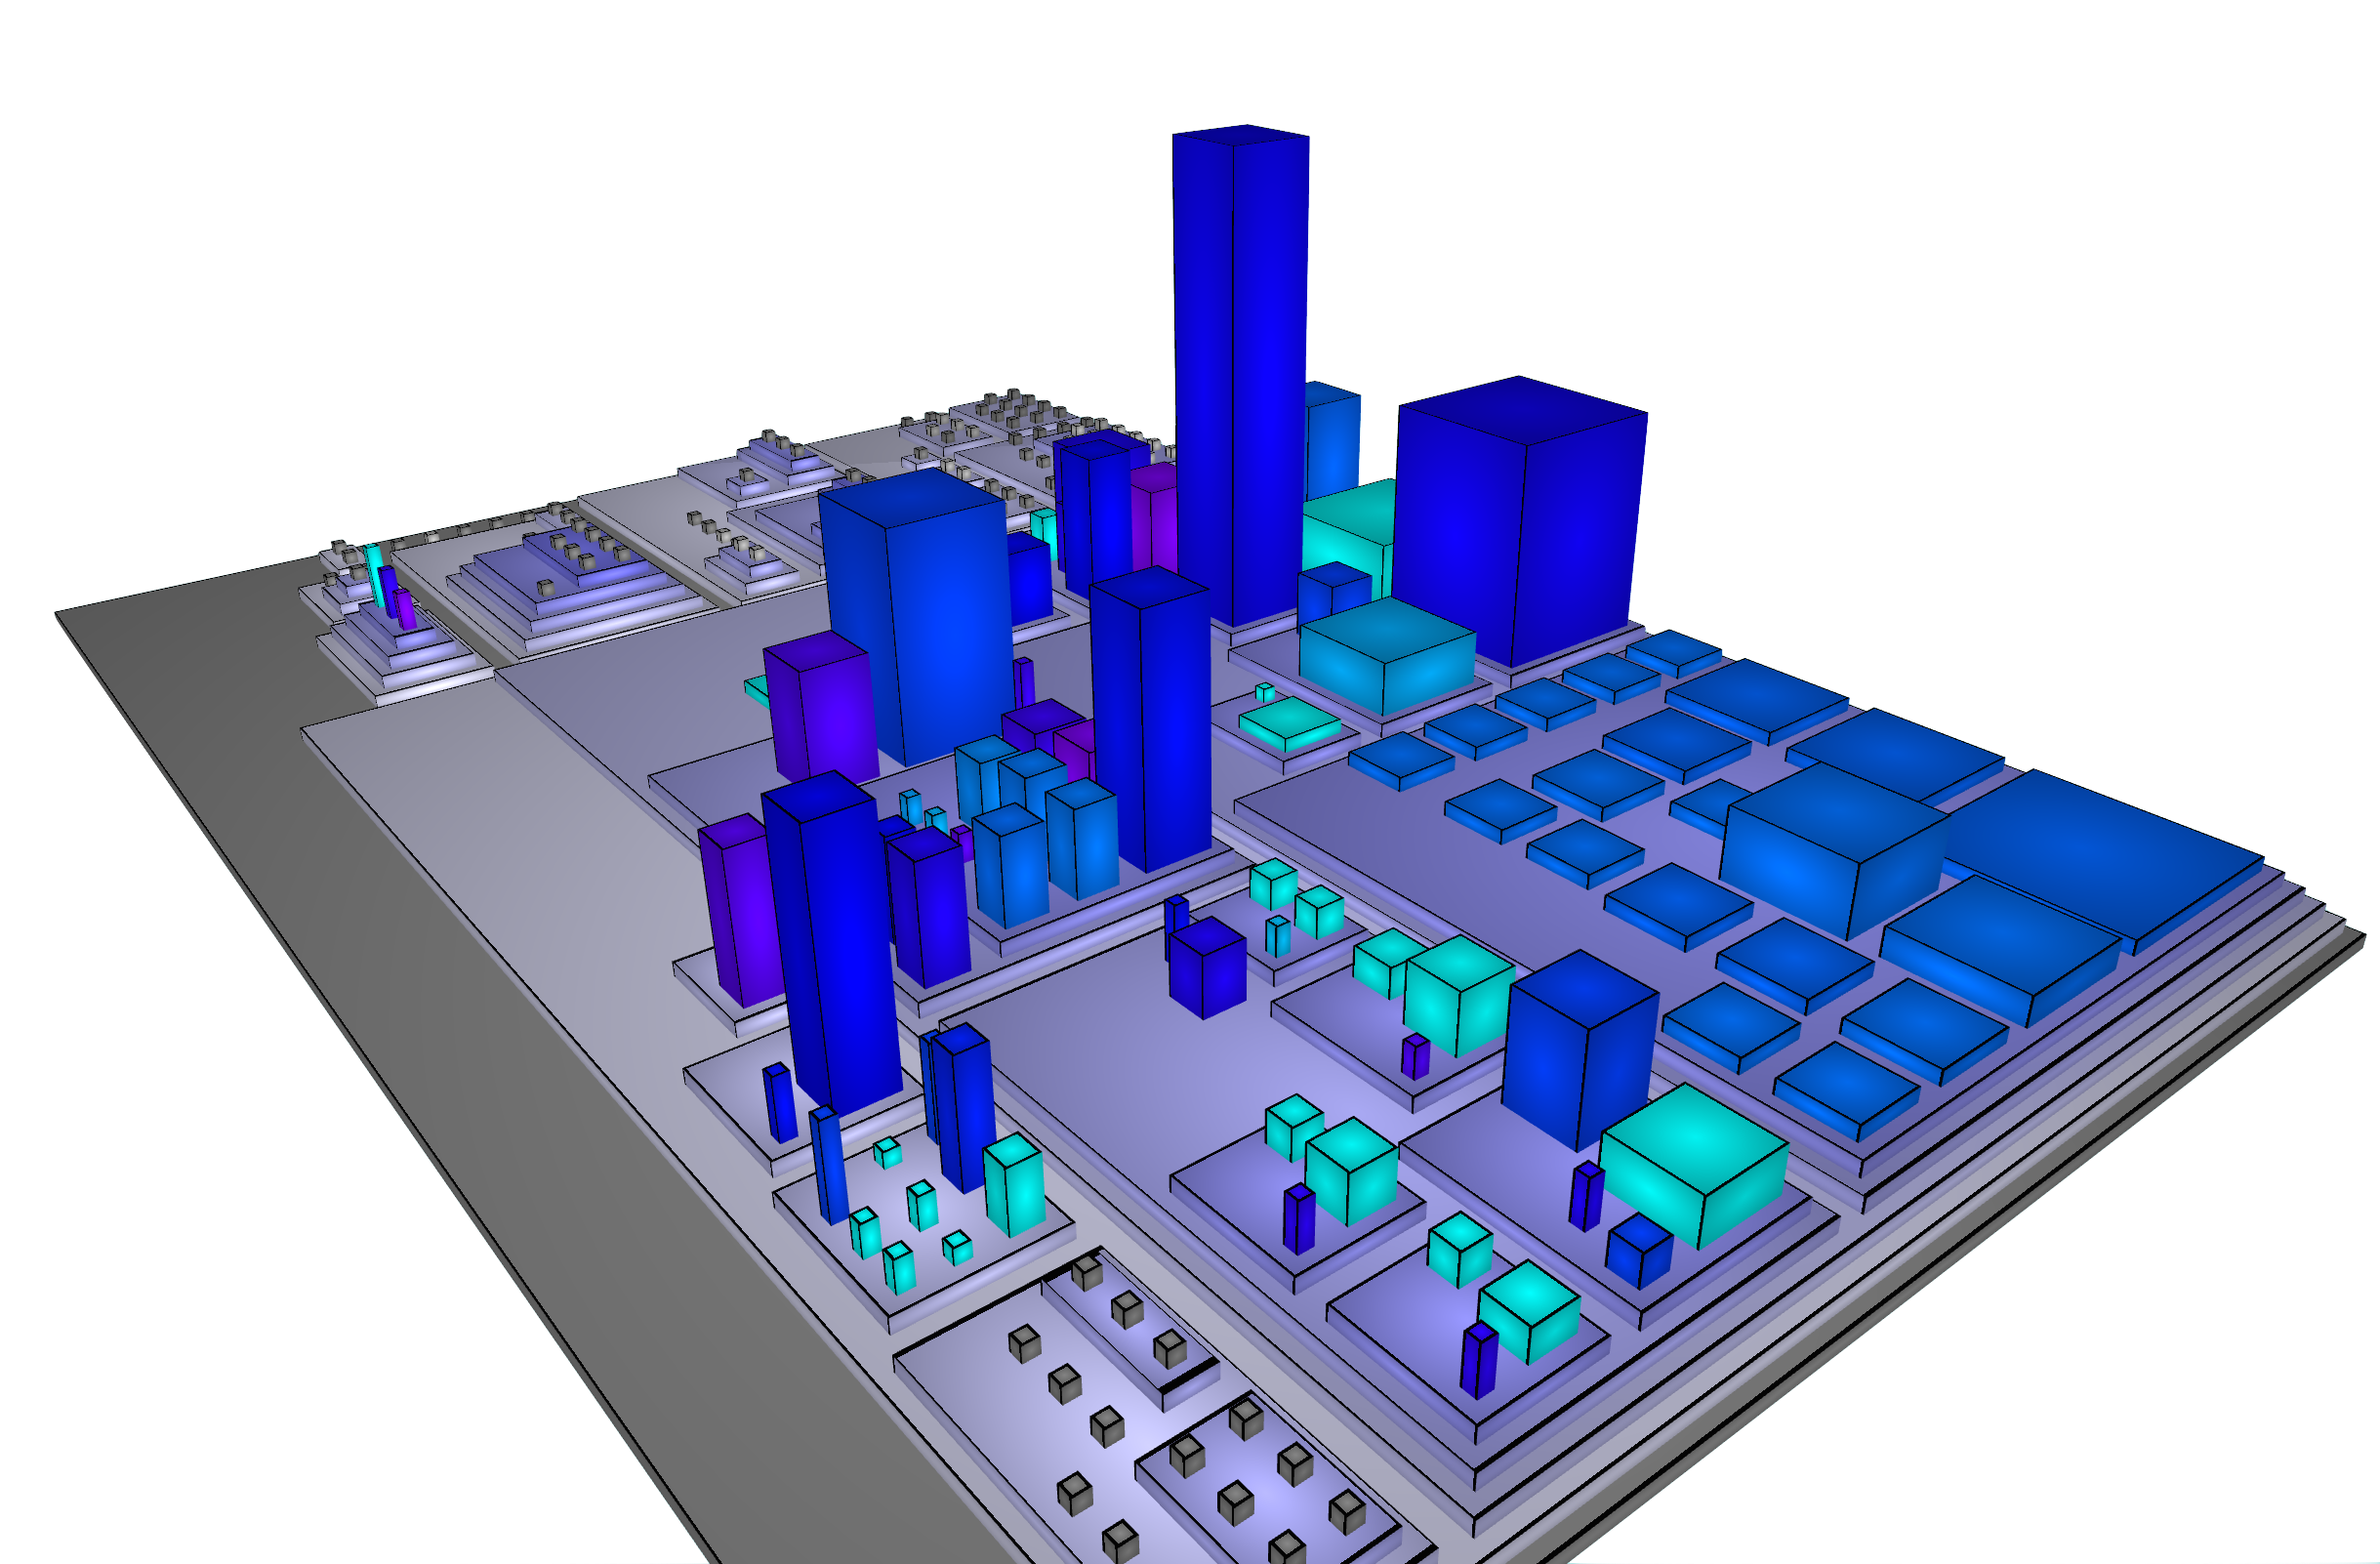
\includegraphics[width=8cm]{images/city1}
\label {myO}
\caption{A first example of a city}
\end{figure}

Starting from this concept, we try to improve this idea of habitability as explained in \cite{vssac} Visualizing Software System as City, where this metaphor is used as a way to allows the developers to get a better understanding of a specific software. \\
As main aim, we thought to help all the people that, coming to the code late during its implementation and development, need to by filled in quickly about all the reference and the information available on it.\\
By doing that, the user can navigate and interact with all the city's components, from the folder (shown as the basement in the render) to all the file that compose the project (shown as building in the render). 


\subsection{Corollary Information} 
Proposition B is a corollary of proposition A if B can be readily deduced from A or is self-evident from its proof, but the meaning of readily or self-evident varies depending upon the author and context. The importance of the corollary is often considered secondary to that of the initial theorem; B is unlikely to be termed a corollary if its mathematical consequences are as significant as those of A. Sometimes a corollary has a proof that explains the derivation; sometimes the derivation is considered self-evident. \cite{wikiCory}\\

For instance, the number of class or the Interface in a file, are information that modifies the structure of the whole project because they are the fiscal parts that compose a system; so they all may be considered corollary information. \\
Instead, on the contrary, the comment has not influenced on the result of a project; it means that they can't be considered corollary information. 
In other words, we can refer to the fiscal part of a project to all the information that you could draw a UML diagram, and the corollary information as all the component that has no design influence on the project, and so are not representable on a UML.\\
The java doc can be used as a simple example of Corollary information  because it is not important for the design proposed, but is extremely useful to understand what the code does. We could also think about the information that is not present, but could be found by using your code. Usually, a software is compose using a different third part library, and it could be helpful to know how much information are available about a call of that particular library because this information gives a better understanding of the code that we are working on. 
The corollary information isn't essentially useful to understand the struct of a system but can give a "normal human readable information" related to its structure.

\subsection{Importance of code related information} 
We can't remove the information related to the code during the visualization process because they give as an intuitively way to understand the topology of the project, and are useful to get a metric unit to better understand what the information coverage means.\\ It's cool to know how much java doc you have respect to a file, but if you don't know the characteristics of that file, you can't say if the documentation is enough or not. Is also useful to use the purely code relation information to have a main idea about the struct of the system, in which package there are more concentration of classes or methods and for highlight design problem.
 

\subsection{Document Structure} 
In section 2 we present the related work. We are going to analyze the functionality of system like Cube8 and we explain briefly how stormed works since is use in this project.
Then we explain the approach used and the different metrics that we used in section 3.
In section 4 we show  two different projects and how to use out system and which kind of informations are possible to retrieves.
Finally we conclude with some improvement that will be interesting  to be implemented.


\newpage


  
\section{Related Works} \label{related works}
Cube8 is a mix of two different sectors and works. One is the visualization method for a software system and the other one is the way to get the corollary information.\\

Program Comprehension through Software Habitability \cite{programComp} propose a city metaphor in which there are a fix number  of building type such as Skyscraper, Office building, Apartment Block,mansion and House. They propose two mapping: Boxplot-based Mapping and Threshold-based Mapping. Also is using a box-packing algorithm to visualize the city.  We are using the same idea of box-packing to organize the city. We also apply the same city metaphor: classes are representing as building located in city districts which in turn represent packages. \\The color meaning is completely different color meaning since we have to visualize different information. In those paper they are concentrate about the structure of a software, here we would like to visualize the coverage information. We still allows the developer to get an idea about other software propriety like classes and interface apply different metrics and therefore generate a new city.The size of the building are code dependent, this allows a better understanding about the system. \\ \\
Visualize Software system as Cities \cite{vssac} is also propose a 3d environment in which the software system is represent as a city, whit different class of buildings. It's also implements a way to navigate and interact with the system.is possible to select any artifact and interact with them, spawning complementary views,  a tagging system and a query system.\\
In Cube8 we have only some of this feature like a basic query system that allows to search for  file name and perform different actions. Is also possible to read the code and navigate through the information found on the web related to a particular building.\\ \\


The StORMeD \cite{stormy} gives a dataset of JSON files, one for each discussion that contain an H-AST about the discussions. The discussion parsing happens in two different step:the former consist into  HTML tag rules to extract the information unit. The latter concern the effective use of the  heterogeneous island grammar.This approach is an extension of Bacchelli \cite{Bacchelli}.  
 We are using simply this dataset to compute the information coverage of the system.

 




\pagebreak
\section{Approach} \label{approach}

\subsection{Introduction}


\subsection{Information Strictly related to the code}
As describe in the introduction we are used code related information to give to the user a better understanding about the locality of your code. To demonstrate this concept you can see two render about the same code. For simplicity we used a huge system that consist of two classes. ClassA has 4 methods and ClassB has 4 method and the same number of fields. We have to find which class need more documentation. The Java Doc, is express in percentage respect the number of method. The color goes from light blue to purple: light blue represent the minimum and purple the maximum. In the figure \ref{fig:strictly:a} , we can see that the big box at left as full documentation, instead, the right one has less. Therefore we found the class that need more documentation (classA) in an easy way. Suppose you have to use the figure \ref{fig:strictly:b}, it has more information not related to the code and has only the method count as code related information. The city become unusable since you can not determinate which is the class A and the class B since the only difference is on the number of fields! Later in this chapter we are going to analyze more in detail color system and the meaning of the used metrics.
\begin{figure}[h]
\centering
\subfigure[Mapping as Width:N of method, height: Number of field, color: javaDoc ]{
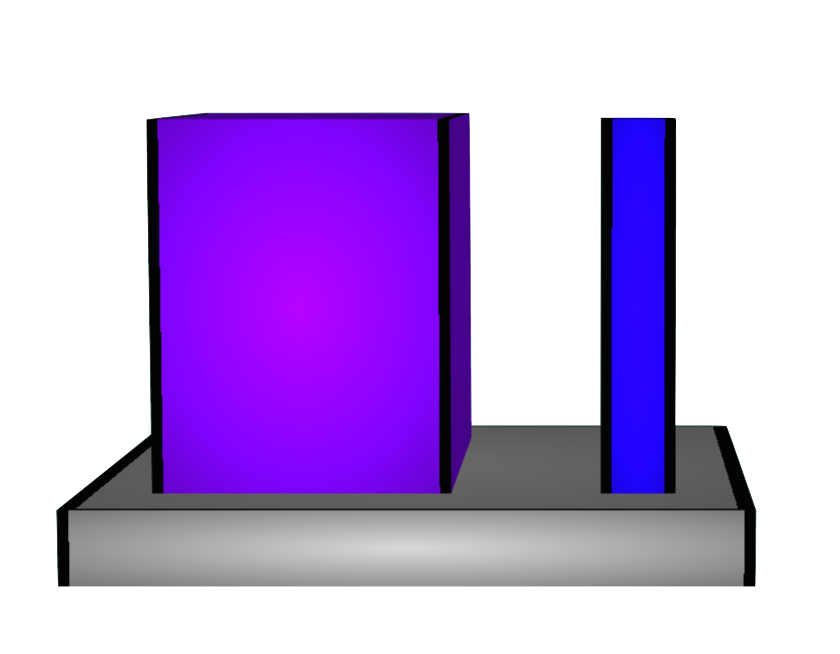
\includegraphics[width=.45\textwidth,height=4cm,keepaspectratio]{images/correctC}
\label{fig:strictly:a}
}
\hspace*{\fill}
\subfigure[Mapping as Width:Discussion count, height: Java doc, color: N of method ]{
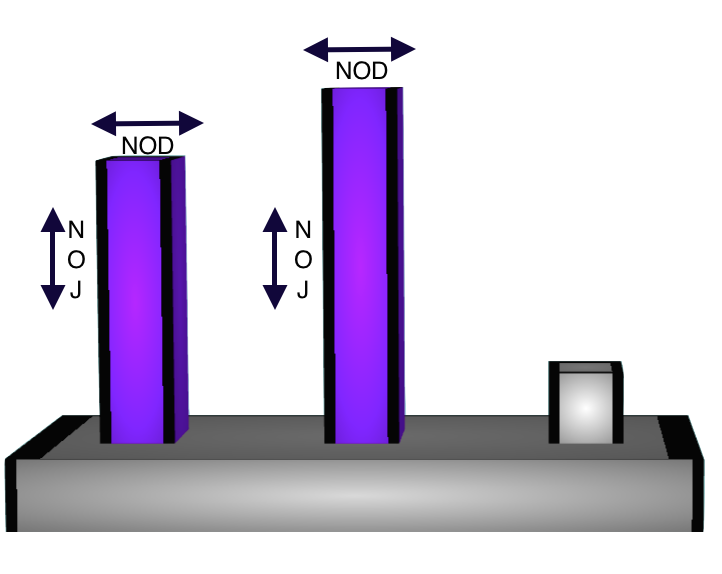
\includegraphics[width=.45\textwidth,height=4cm,keepaspectratio]{images/wrongC}
\label{fig:strictly:b}
}

\caption{Information Strictly related to the code}
\label{fig:strictly}

\end{figure}

\subsubsection{Class and Interface}

The classes and  interface are another metrics that we add to our tools. Remember that the basic building represented is the source file.  By the Java Code Conventions \cite{oracle}  \" Each Java source file contains a single public class or interface. When private classes and
interfaces are associated with a public class, you can put them in the same source file as the public class\". This mean that we could have more classes in a single source file and therefore could be useful to have a metrics that give to the analyzer the ability to find this relations.

\begin{figure}[h]
\centering

		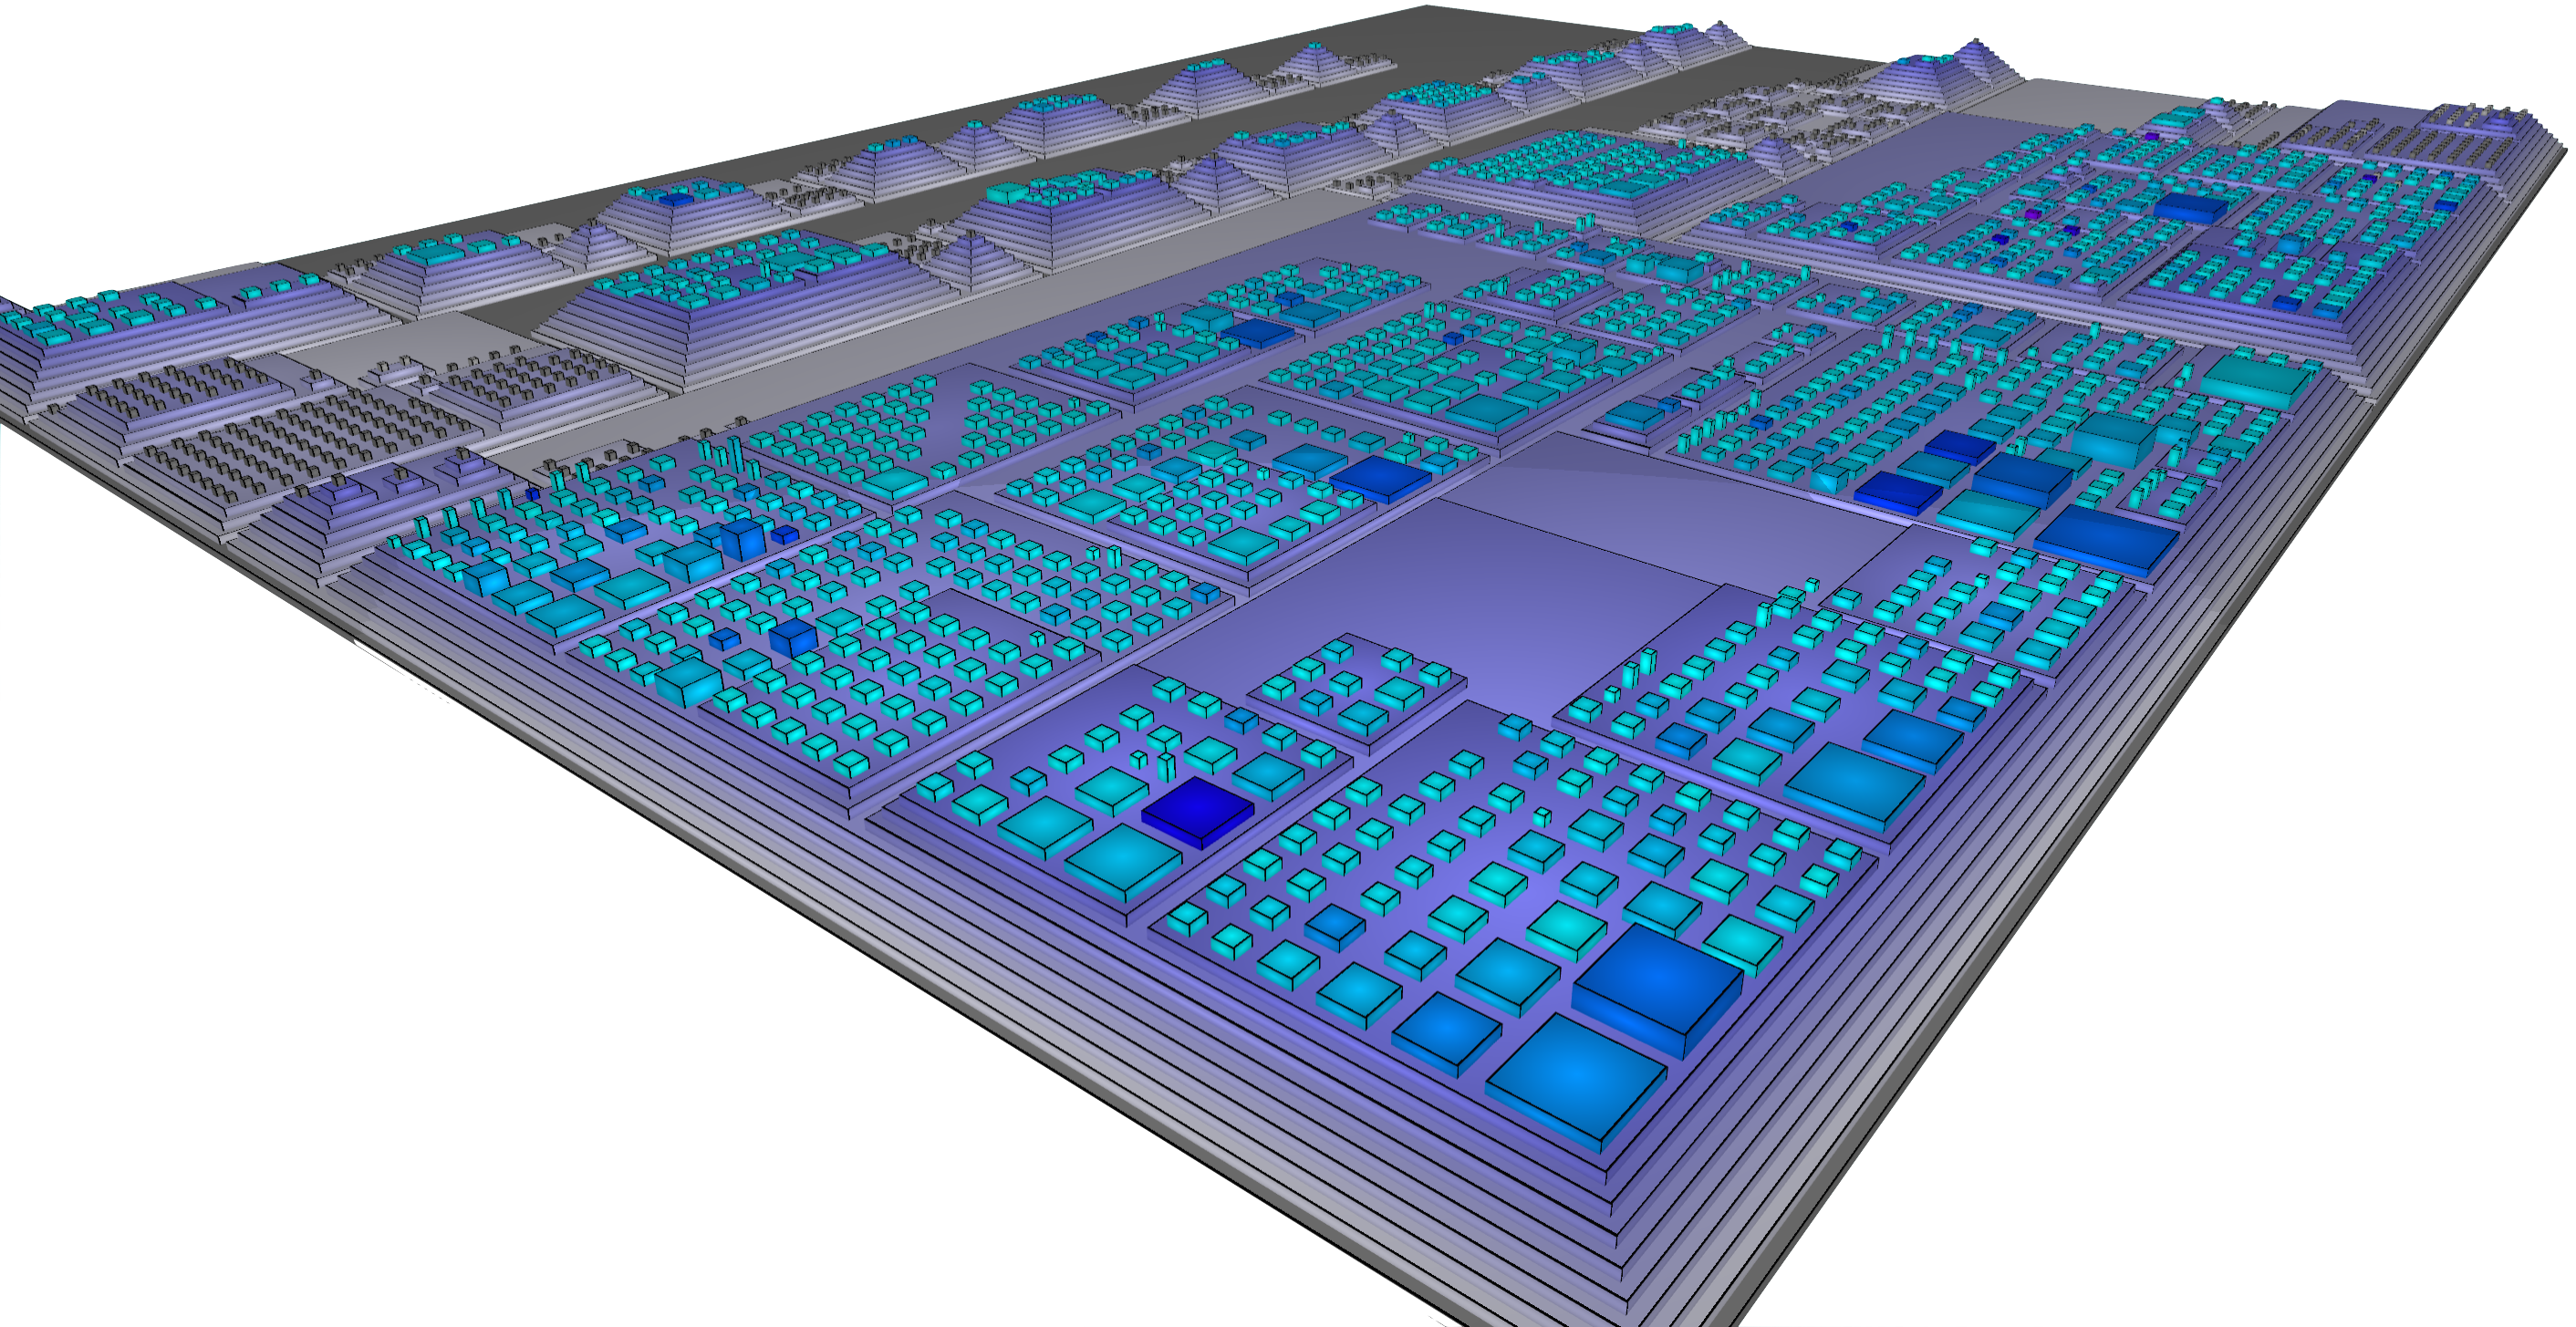
\includegraphics[width=.60\textwidth]{images/ClassesAndInterfaces}
	\label{fig:classInterface}
	\caption[Classes and Interfaces Mapping]{Mapping as Width:N of Class, height: Number of interface}
	
\end{figure}

This is an example where we analyze this two concept in a big project.
As you can see there are a few classes that could need some check to make sure that this design  principle is respected.

\subsubsection{Methods  and Fields}
Method and field are the main component that compose a class or interface. In the tools we are using this two measure to map  the size of the buildings. The reason is that this two concepts give the correct granularity to have a better understand about the system.\\
We can also identify a potential God Class that has a hight number of method  or a Data Class that has a hight number of field and a few  methods.
Let's get an example. We using the same project as before.
\begin{figure}[h]
	\centering
	
	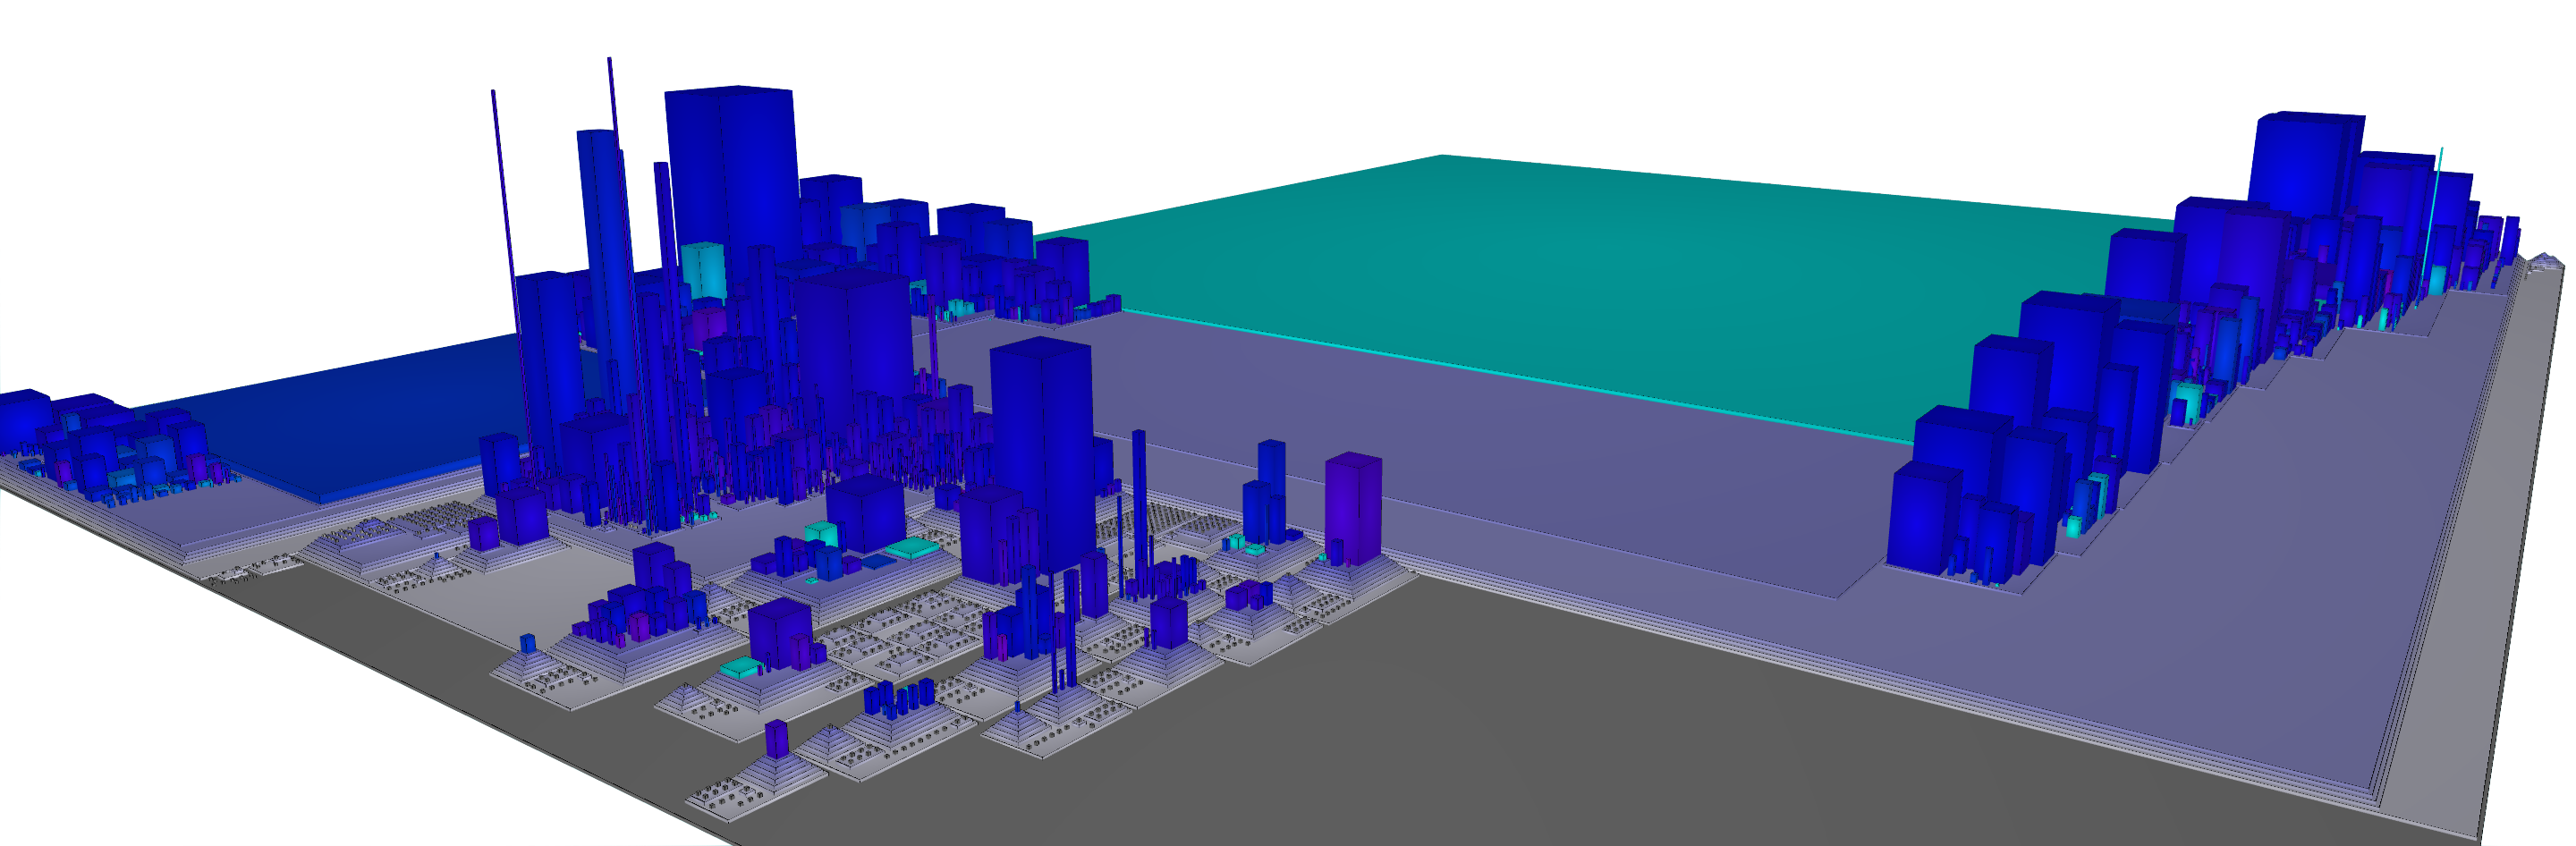
\includegraphics[width=1\textwidth]{images/fieldAndMethod}
	\label{fig:classInterface}
	\caption[Fields and Methods Mapping]{Mapping as Width:N of Fields, height: Number of Method}
	
\end{figure}

It's easy to see that there is a  flat an big building that could represent a Data Class and  there are two thigh and height building that could represent a God Class. In this case the both candidate for the god Class are tests. Instead the Data Class has really  686 fields.
    
\pagebreak
\subsection{Information Not Strictly related to the code}
The information not strictly related to  code are the core of this paper. As we sow before, there already exist tools that allows the visualization of a system as a city, and they does a lot of computation around strict related information. What we interesting, instead, is the amount ok knowledge that are available about a given system. This knowledge are meaningful to get an idea about the complexity of understanding a software system and where it should be use more effort.At the same time it  could  be use as a monitor for the developers to understand which part of their code need more information.  


\subsubsection{Java Documentation}
Collecting and visualizing the java doc was the first step of the process to collecting the coverage information since it is integrated on the code and he doest require any  particular computations. It cover an important role in the process of understanding the functionality of a given code since is written directly by the developers and should be use in each method, field and class definitions.
With this computation unit is possible to visualize the documentation state of a project. We usually map the java doc using the color; it is collect only the method documentation since we claim that was a good level of granularity. The class documentation was not enough, it gives only a global view of the functionalities.

\begin{figure}[H]
	\centering
	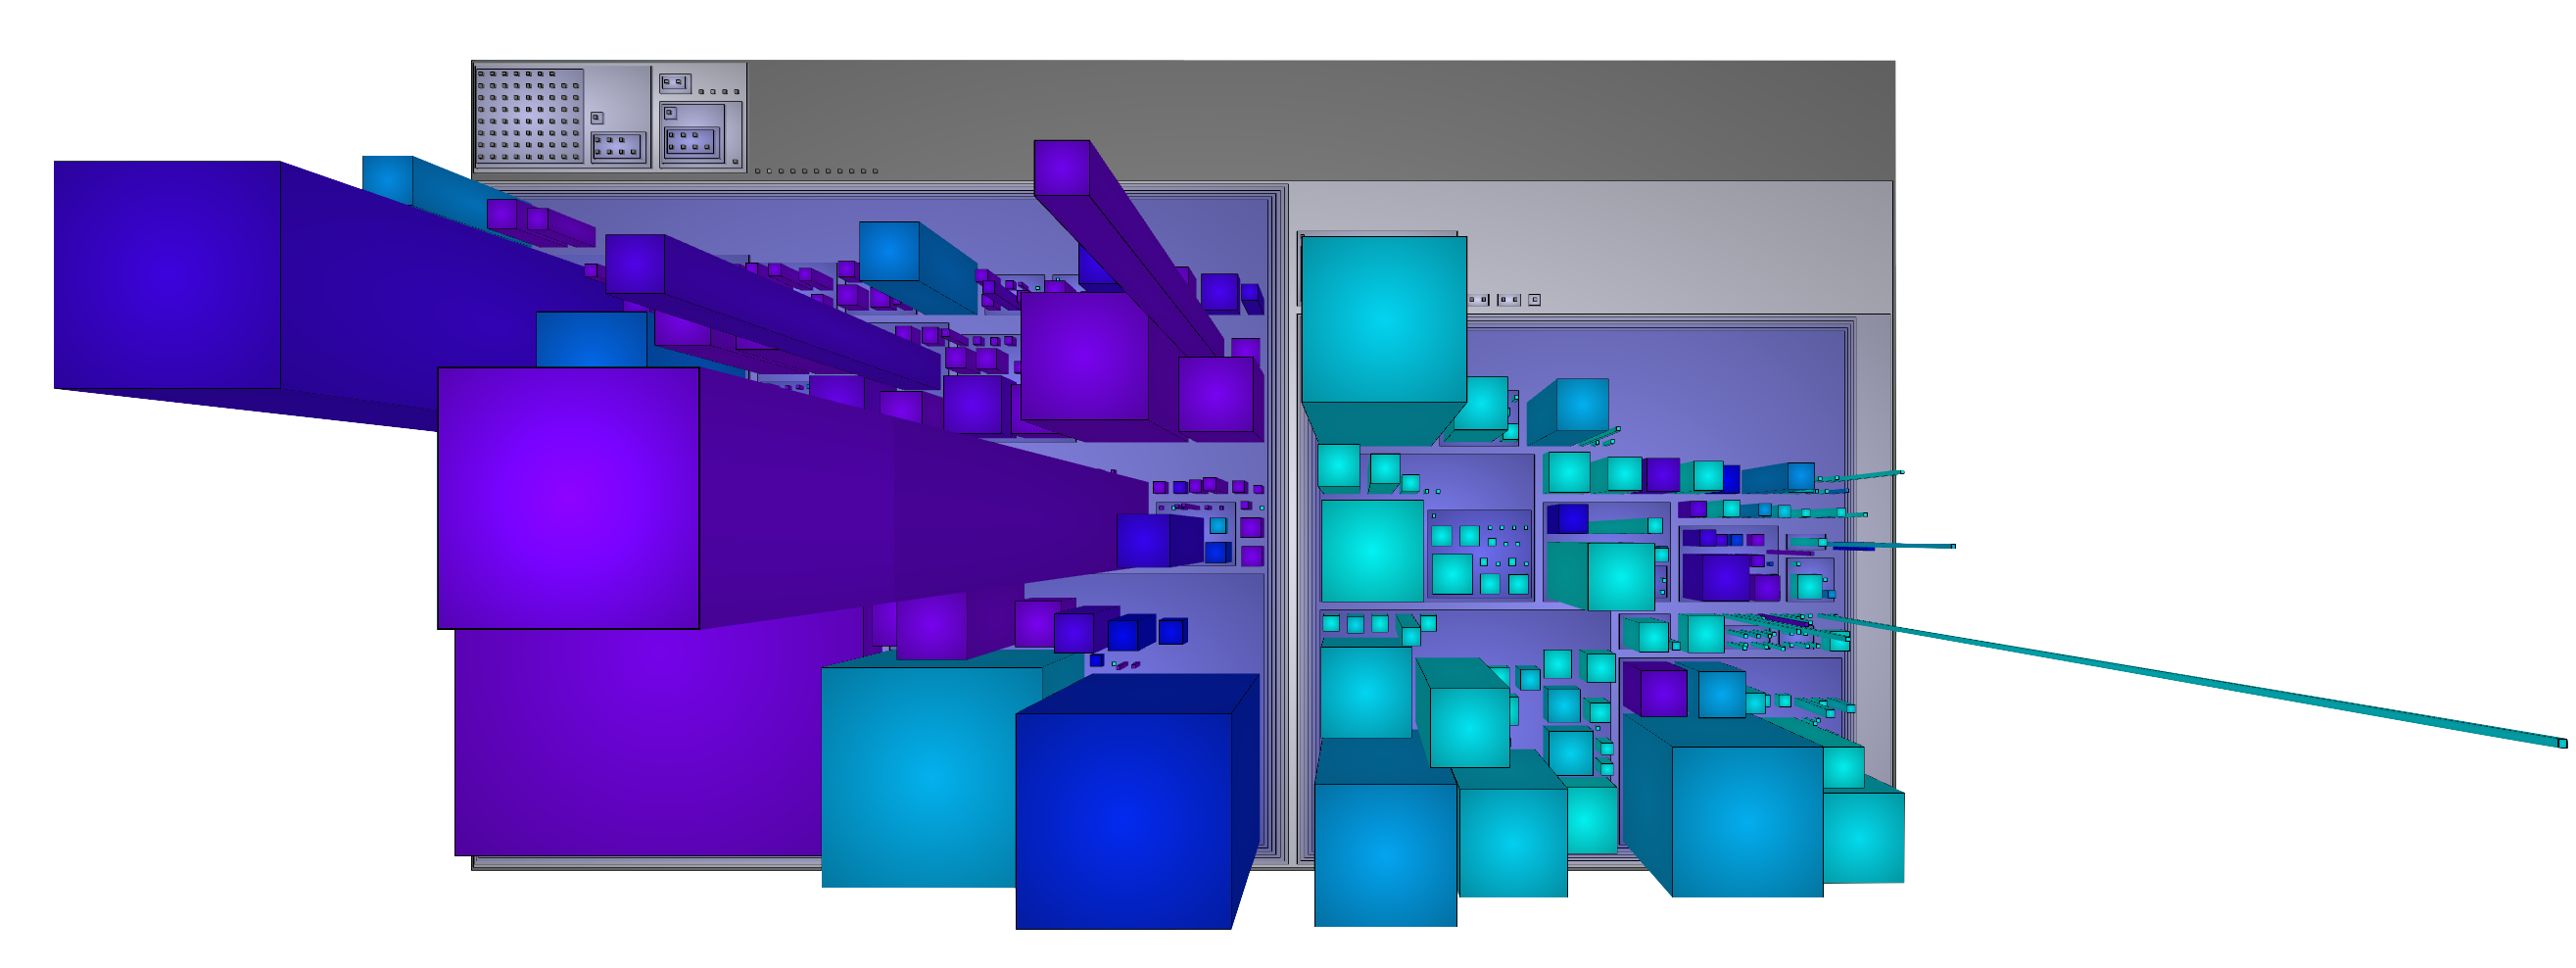
\includegraphics[width=1\textwidth]{images/javaDoc}
	\label{fig:javaDoc}
	\caption[Java Documentation Mapping]{Mapping as Width:N of Fields, height: Number of Method,Color: Percentage of documented methods}

\end{figure}

Figure \ref{fig:javaDoc} is example of a city in which the color represent the percentage of documented methods.The project is the apache common-lang . Is very interesting to see that half of the project has a documentation coverage greaten that the 80\% and in the other one is very rare. In reality this is a common case since a lot of project does't document the tests.
To help the analyzer to understand the documentation coverage we also provide a package base coloring system. In which the color of each package is the average of the child component. In  this case it look like figure \ref{fig:OnlyPackage}

\begin{figure}[H]
	\centering
	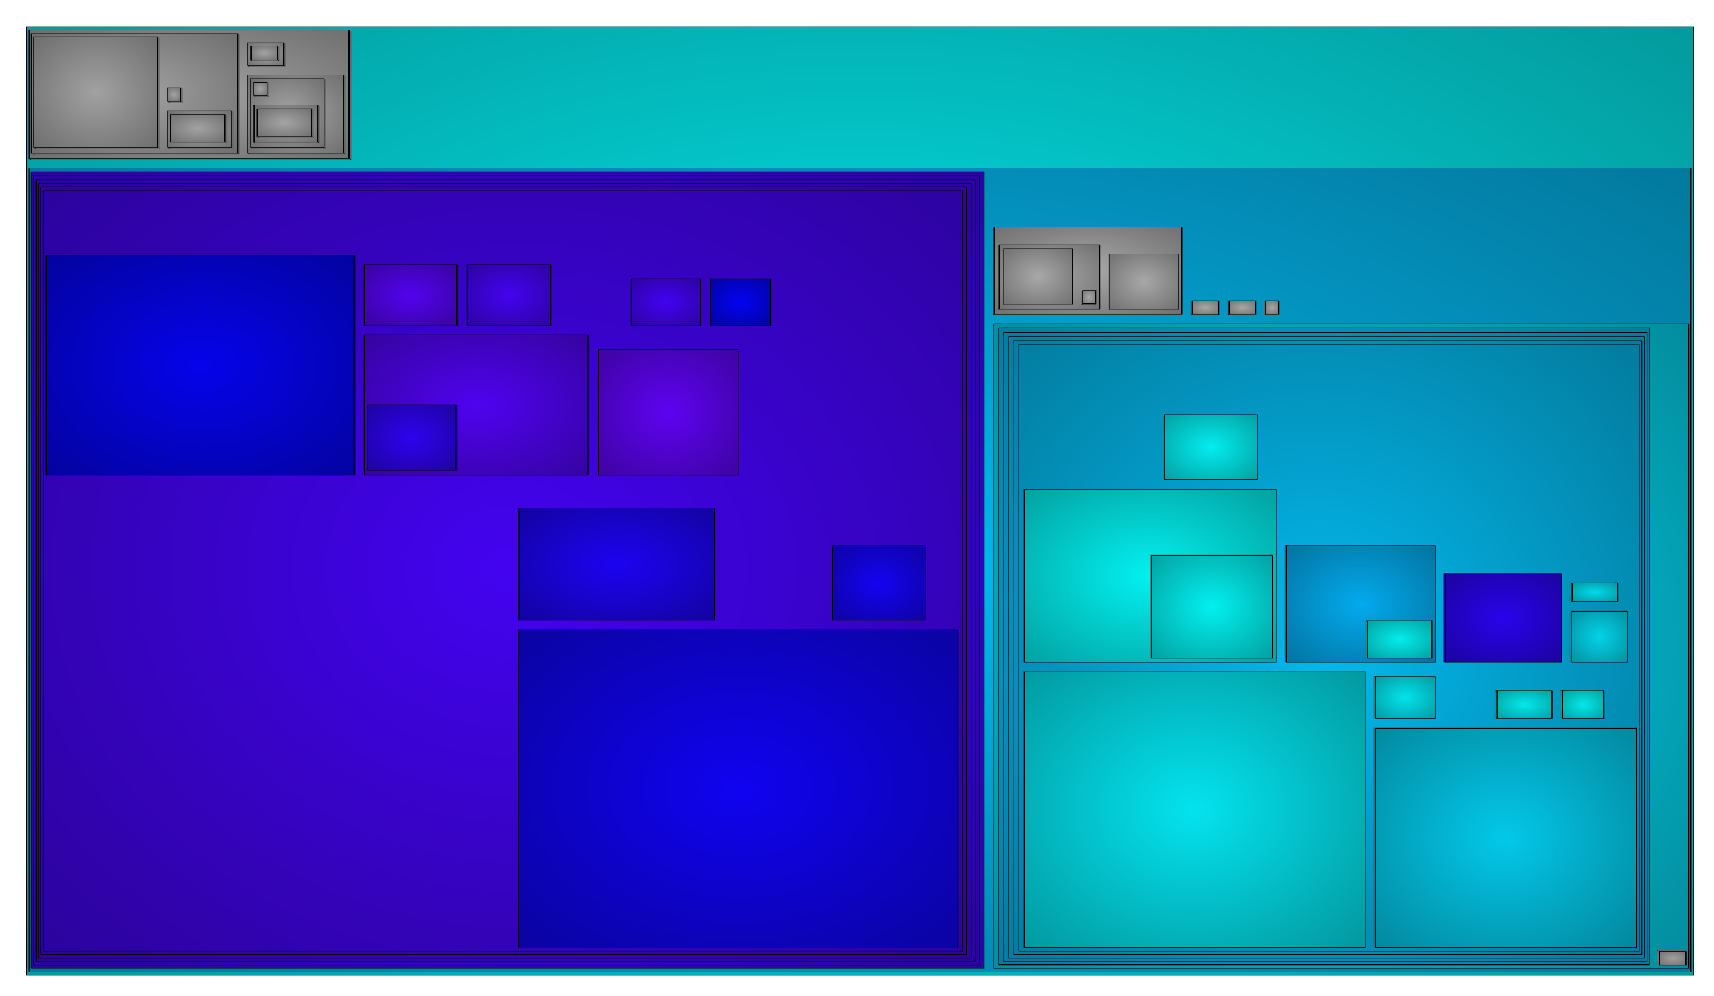
\includegraphics[width=0.5\textwidth]{images/javaDocOnlyPackage}
	\label{fig:OnlyPackage}
	\caption[Java Documentation Mapping Only Package]{Mapping as Width:N of Fields, height: Number of Method,Color: Percentage of documented methods}
\end{figure}


\subsubsection{Stack Overflow  Discussion}





\subsection{Merge Code Related information with Corollary Information}

\subsubsection{Corollary Information and  Methods}

\subsubsection{Percentage and Absolute Numbers of informations}

\subsubsection{Using Java Doc and Discussion together}


\subsection{Colors}

\subsubsection{Corollary Information Color meaning}

\subsubsection{Code related Color meaning}

\subsection{System Architecture }


\section{Evaluation} \label{evaluation}

\subsection{Introduction}

\subsection{Tomcat}


\subsection{ITextPDF}



\section{Conclusion} \label{conclusion}





%%%%%%%%%%%%%%%%%%%%%%%%%

%\subsection{General issues}
%
%Latex is not so complex. If you aren't familiar with it just spend some time in googling for latex commands (e.g. font formats, tables, figures, items,\dots).
%
%\subsection{Getting started}
%In order to use the bachelor thesis template, be sure that the following files are present in your working directory:
%\begin{itemize}
%\item usiinfbachelorproject.cls (The latex template)
%\item logo-info.pdf (The logo figure)
%\item references.bib (The references file)\\
%\end{itemize}
%
%\subsection {Compilation issues}
%
%If you are not familiar with Tex, I advise you to download TexShop for Mac OS.\\
%To include the references and display them in the final pdf, you have first to typeset this file with \textit{LaTex} (ComboBox upper left, if you use TexShop), then with \textit{BibTex} and finally again with \textit{LaTex}.\\
%In order to resolve figures/table/\dots~references you have to run 2 times the (latex) typeset.
%
%\subsection {Document structure}
%
%Some basic sections:
%\begin{itemize}
%\item Introduction (including Motivation)
%\item State of the Art
%\item Project requirements and analysis
%\item Project design (top-down)
%\item Implementation issues (bottom-up)
%\item Tests (methodology, results, comments)
%\item Conclusions and future work or possible developments
%\end{itemize} 
%
%\subsection {Some examples}
%
%\textbf{Figure ~\ref{fig:USILogo}} shows how to insert figures in the document.
%
%\begin{figure} [h]
%\centering
%
\includegraphics[width=0.5\textwidth]{logo-info.pdf}
%\caption{Caption of the figure}
%\label{fig:USILogo}
%\end{figure}
%
%\noindent\textbf{Table ~\ref{tab:numbers}} shows how to insert tables in the document.
%
%\begin{table}[h]
%\centering
%\scalebox {0.8} {
%\begin{normalsize}\begin{tabular}{l|lll}
%\textbf{Col 1} & \textbf{Col 2} & \textbf{Col 3} & \textbf{Col 4}\\
%\hline
%1 & 2 & 3 & Goofy\\
%4 & 5 & 6 & Mickey



%\end{tabular}
%\end{normalsize}
%}
%\caption{Caption of the table}
%\label{tab:numbers}
%\end{table}


%%%%%
\newpage

\bibliographystyle{abbrv}
\bibliography{references}

\end{document}